\documentclass[11pt,compress,t,notes=noshow, aspectratio=169, xcolor=table]{beamer}
% deactivate beamer navigation
%\setbeamertemplate{navigation symbols}{}
%\usepackage{geometry}
%\geometry{papersize={180mm, 135mm}, top=-1.5mm} % 210mm, 297mm

\usepackage{multicol}
% set path of iml lecture here, e.g., relative to the current dir
\newcommand{\pathiml}{../}
\usepackage{\pathiml/style/lmu-lecture-bak}
\usepackage{pax}
\setbeamertemplate{frametitle}{\expandafter\uppercase\expandafter\insertframetitle}
%\useoutertheme{metropolis}
% remove section slides
\AtBeginSection[]
{
  \begin{frame}<beamer>
    \frametitle{Introduction to IML}
    %\begin{multicols}{2}
    \tableofcontents[currentsection]
    %\end{multicols}
  \end{frame}
}
% includepdf slides, pagecommad will set counter for framenumber
\usepackage{pdfpages}
\includepdfset{trim=0mm 0mm 42mm 0mm, pagecommand={\global\setcounter{framenumber}{\value{page}}}}
%trim=left bottom right top,clip
% trim=0mm 6mm 0mm 0mm, offset=0 15,
% add footer:
\usepackage{framed, color}
\usepackage{xcolor}
%\iffalse
\setbeamertemplate{footline}[text line]{%
    \noindent\hspace*{\dimexpr-\oddsidemargin-1in\relax}%
     \colorbox{white}{
     \makebox[\dimexpr\paperwidth-2\fboxsep\relax]{
     \color{black}
     \begin{minipage}[c][2ex][c]{0.5\linewidth}
       \secname
     \end{minipage}
     \hfill\begin{minipage}[c][2ex][c]{0.5\linewidth}
       \flushright
       \insertframenumber{}~/~\inserttotalframenumber~~
     \end{minipage}
     }}%
  \hspace*{-\paperwidth}
}
%\fi


\begin{document}
\setbeamercolor{background canvas}{bg=}

% General remark: hyperlinks in included pdfs are not clickable anymore in the combined pdf unless you use pax to extract annotations from original files and complile this file locally (see https://tex.stackexchange.com/questions/497624/merging-multiple-pdf-files-without-breaking-hyperlinks)


\section{Introduction and Motivation}
%% INTRO
\includepdf[pages={3, 6}]{../../lecture_iml/slides-pdf/slides01-intro-motivation.pdf}
% 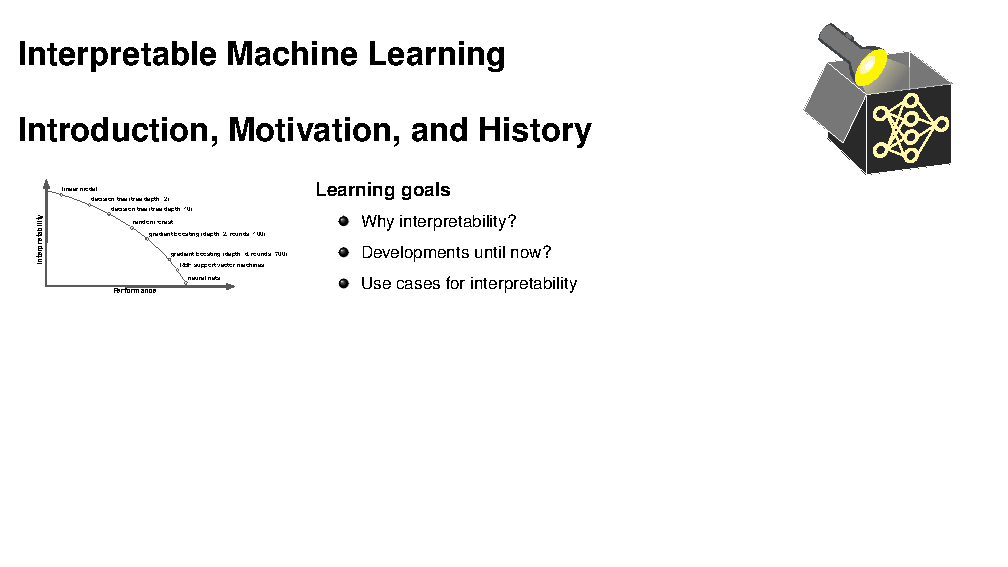
\includepdf[pages={1}]{../../lecture_iml/slides-pdf/slides01-intro-motivation.pdf}
% 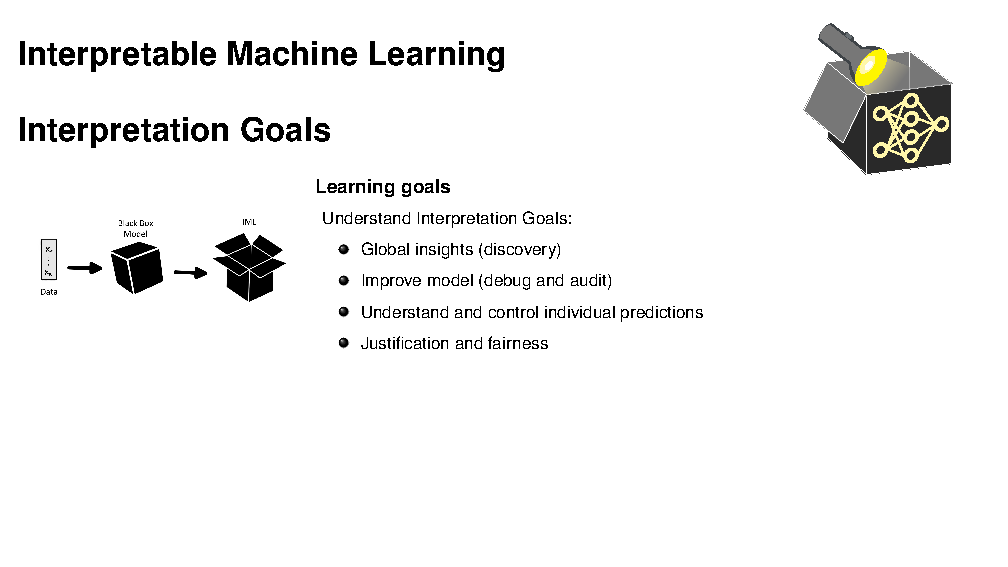
\includepdf[pages=-]{../../lecture_iml/slides-pdf/slides02-intro-goals.pdf}
\includepdf[pages={2-4, 13}]{../../lecture_iml/slides-pdf/slides03-intro-dimensions.pdf}
%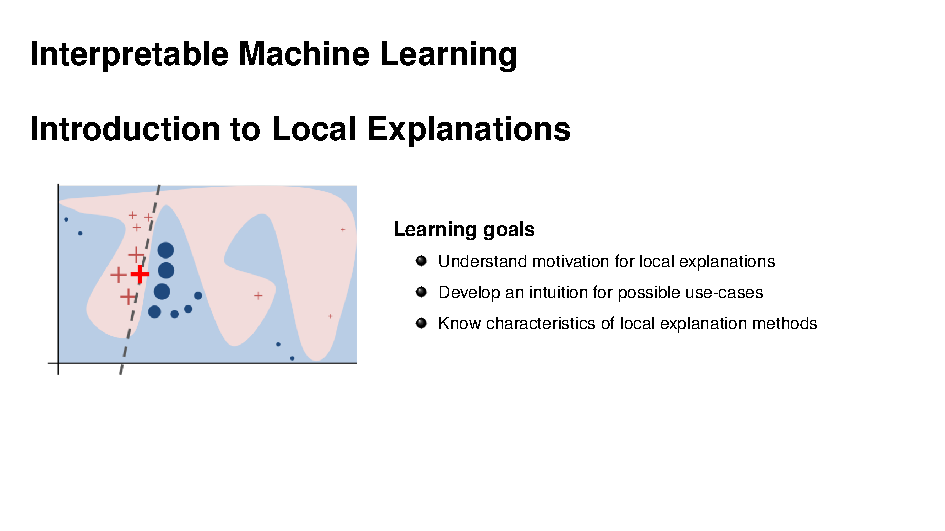
\includepdf[pages={1-7,16-21}]{../../lecture_iml/slides-pdf/slides01-le-intro.pdf}

\section{Feature Effects - ICE and PDP}
%% INTRO FE
\includepdf[pages={2-4}]{../../lecture_iml/slides-pdf/slides01-fe-intro.pdf}
%% ICE Curves
%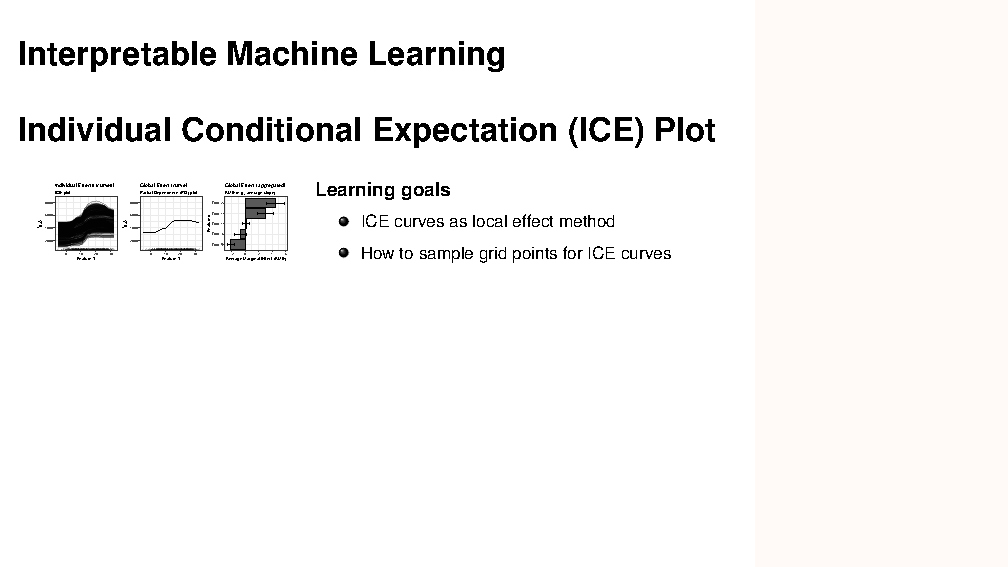
\includepdf[pages={1-10}]{../../lecture_iml/slides-pdf/slides02-fe-ice.pdf}
%% PDP
\includepdf[pages={2-5, 8}]{../../lecture_iml/slides-pdf/slides03-fe-pdp.pdf}
%\includepdf[pages={2}]{../../lecture_iml/slides-pdf/slides04-fe-pdp-comments.pdf}
%\includepdf[pages={12,18,20}]{../../lecture_iml/slides-pdf/slides04-intro-correlation.pdf}

\section{Loss-based Feature Importance - PFI}
%% INTRO FI 
\includepdf[pages={3}]{../../lecture_iml/slides-pdf/slides01-fi-intro.pdf}
%% PFI
\includepdf[pages={2-10}]{../../lecture_iml/slides-pdf/slides02-fi-pfi.pdf} % 14
%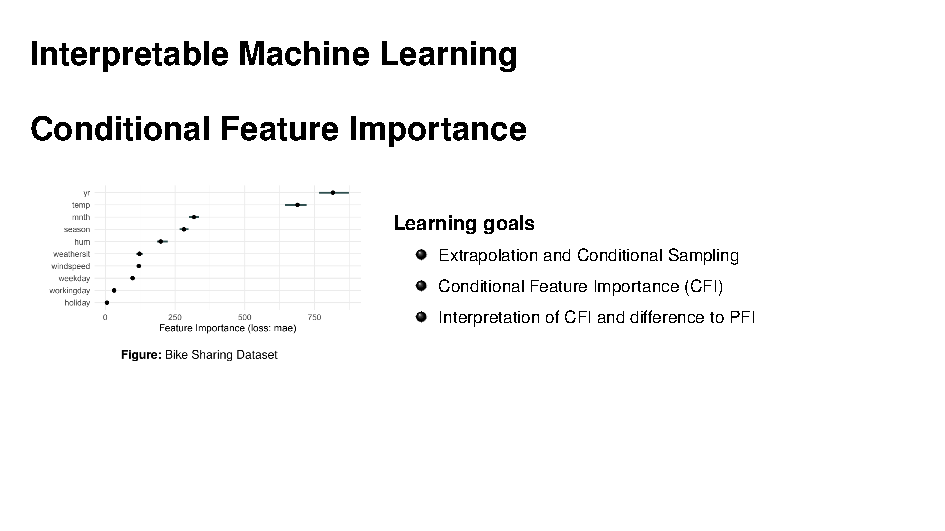
\includepdf[pages=-]{../../lecture_iml/slides-pdf/slides03-fi-cfi.pdf}

%% LIME
\section{Local Explanations - LIME}
\includepdf[pages={4, 7-8, 10-14, 16-20}]{../../lecture_iml/slides-pdf/slides04-le-lime.pdf}
\includepdf[pages={2-4}]{../../lecture_iml/slides-pdf/slides05-le-lime-examples.pdf}
%\includepdf[pages={4, 7-8, 10-14, 16-20}]{../../lecture_iml/slides-pdf/slides04-le-lime.pdf}
%\includepdf[pages={2-4}]{../../lecture_iml/slides-pdf/slides05-le-lime-examples.pdf}

%\includepdf[pages={2}]{../../lecture_iml/slides-pdf/slides06-le-lime-pitfalls.pdf}

\end{document}
